\chapter{Intelligence artificielle et compléments}
\label{chap:chapter_3}
\chapterintro
Lors du précédent chapitre, nous avons abordé les interactions entre la peau et la lumière, ainsi que les dispositifs majeurs permettant l'acquisition d'informations de la peau. Dans la continuité de cette partie nous avons présenté l'étude clinique de référence et les données associées.\par

De nos jours, l’informatique est une ressource omniprésente dans de nombreux domaines d’application. Sa faculté à nous divertir ou encore à nous guider dans nos choix quotidiens personnels et professionnels en fait un précieux allié.\par 

De nouvelles pratiques font leurs apparitions, intégrant la machine au cœur des processus décisionnels. Les disciplines médicales évoluent largement, l’ordinateur permettant de répondre aux besoins croissants de précision et reproductibilité (intra et inter opérateur) et de gain de temps au sein de la pratique clinique. Il s’agit également d’un moyen de formaliser la connaissance au travers d’un outil, qui dans un cadre bien défini, peut être utilisé par des non-initiés.\par

Cette nouvelle partie nous permet de dérouler un peu plus notre plan, en abordant cette fois-ci les systèmes d'intelligence artificielle et comment appréhender leur utilité vis à vis des données que nous avons à traiter.\par
\newpage

\section{Généralités sur l'intelligence artificielle}
La notion \textbf{d’\gls{ai}} est assez souvent contestée, mais se définit plus généralement comme étant « L’ensemble de théories et de techniques mises en œuvre en vue de réaliser des machines capables de simuler l'intelligence humaine »~\textsuperscript{\ref{footnote:ia_larousse}}. Ainsi, la retranscription sous forme informatique de mécanismes de pensée humaine, sont compris dans cette notion.\par

Une vision plus complète de ce terme consiste a décomposer l'\gls{ai} en une discipline composée de sous domaines possédant chacun leurs spécificités, comme schématisé sur la \Cref{fig:scheme_overview_ia}. Ainsi, le terme \textbf{d'apprentissage automatique} ou de "Machine Learning" caractérise un premier sous champs de l'\gls{ai} et sera employé pour qualifier l'utilisation de mécanismes statistiques dans le but de générer des règles, à partir de données d'apprentissage. Ces données, souvent complexes, il sera souvent nécessaire de laisser l'humain intervenir pour extraire l'information pertinente à l'accomplissement de la tâche souhaitée. Enfin, le terme \textbf{d'apprentissage profond} ou de "Deep Learning" va désigner un sous champ de l'apprentissage automatique, dans lequel des couches de prises de décision vont permettre d'augmenter la complexité des relations entre les données d'entrée et les tâches.\par

\addtocounter{footnote}{1}
\footnotetext[\thefootnote]{Source : Encyclopédie Larousse. \label{footnote:ia_larousse}}

\begin{figure}[H]
    \centering
    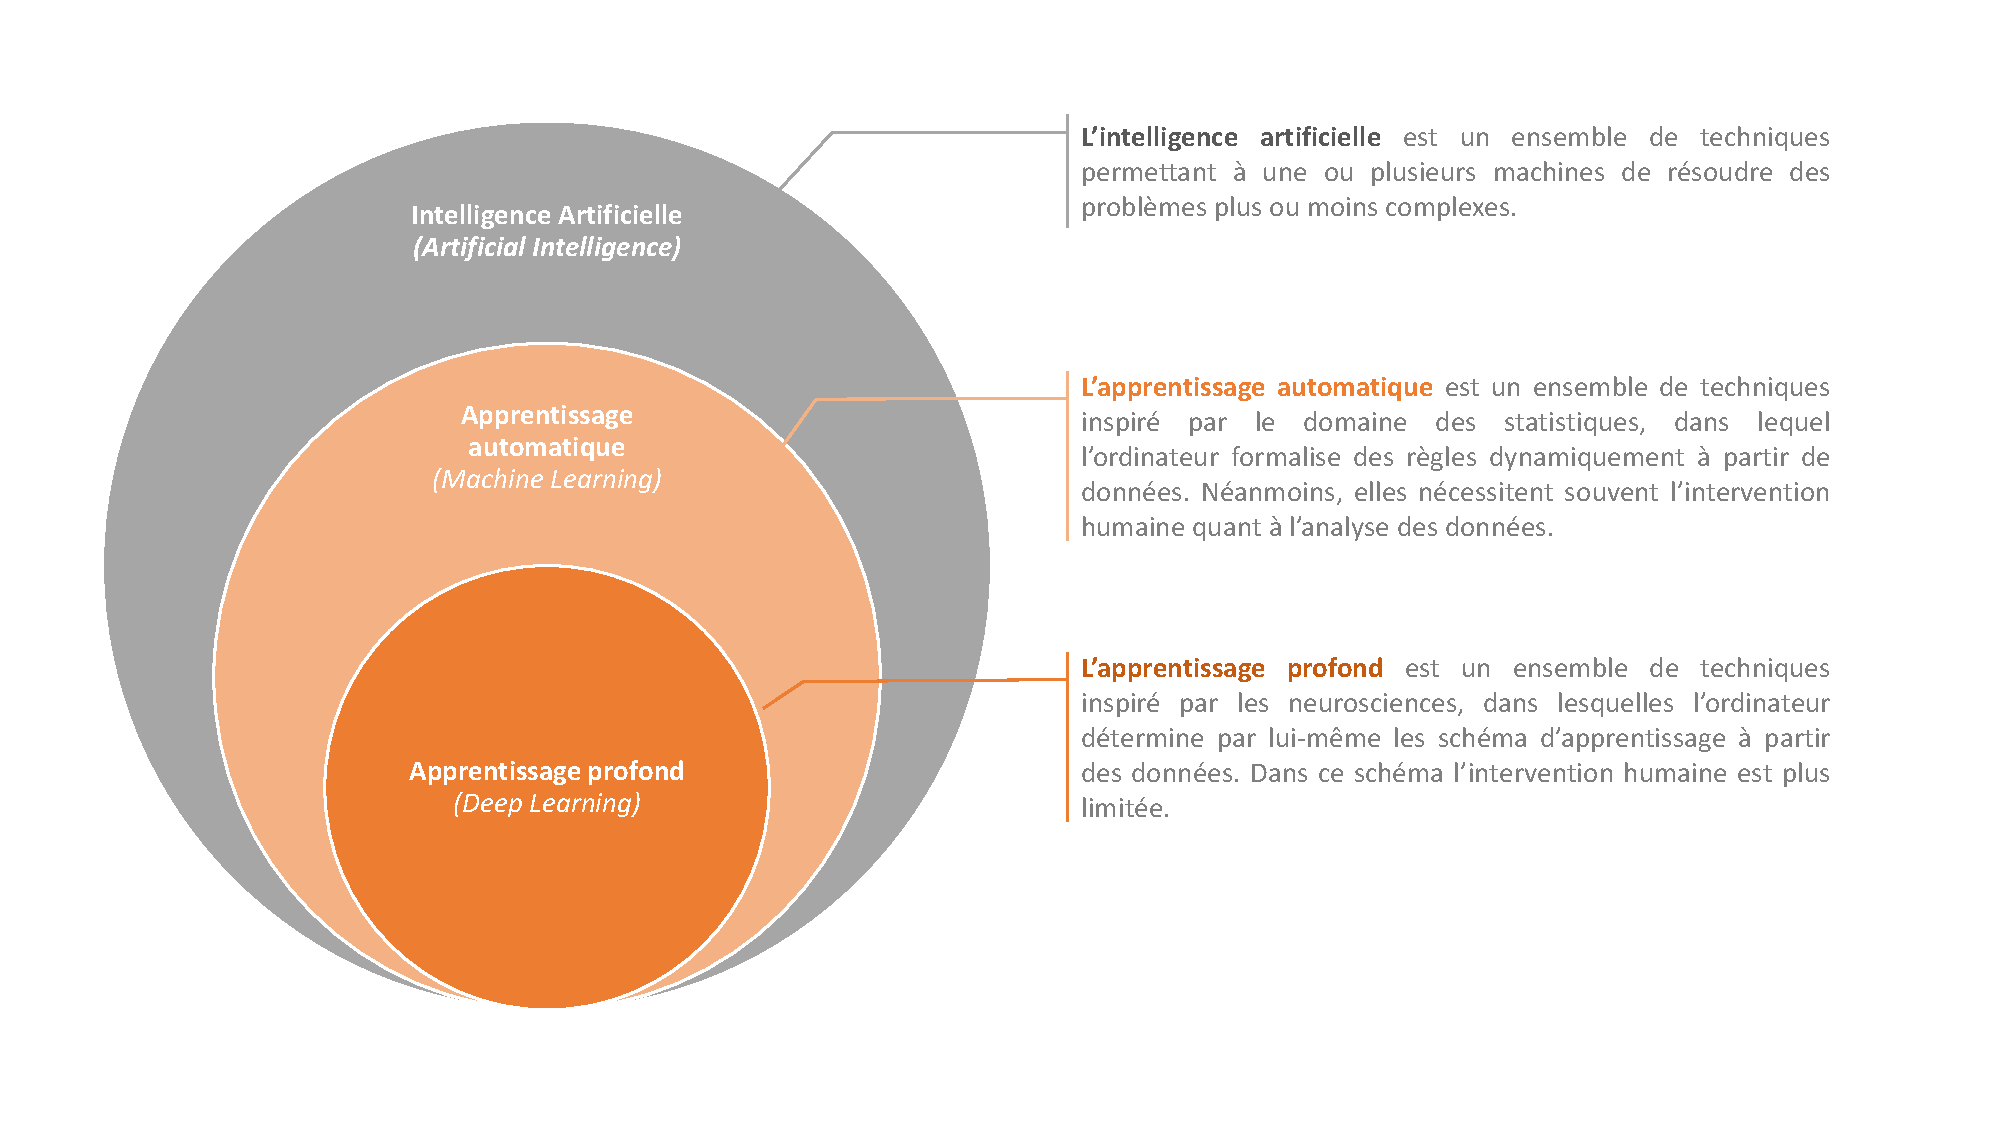
\includegraphics[width=\linewidth]{contents/chapter_3/resources/scheme_overview_ia.pdf}
    \caption{Représentation des relations entre "Intelligence artificielle", "Apprentissage automatique" et "Apprentissage profond".}
    \label{fig:scheme_overview_ia}
\end{figure}\par

Cette partie a pour vocation d’amener à la compréhension générale des courants d’\gls{ai}, qui permettent la résolution de problématiques variées, mais surtout la résolution de certains problèmes de dermatologie. Nous décrirons dans une première partie, les approches par apprentissage. Ces deux catégories se référent directement à notre thématique, à savoir l’analyse de lésions assistée par l’imagerie optique.\par

\section{Approches par apprentissage}
Ce courant a été « évoqué » en 1948 par Alan Turing, son idée était de proposer des « machine à apprendre susceptibles de construire elles-mêmes leurs propres codes » \cite{Turing1950}. En 1959, Arthur Samuel  formule une première définition des approches par apprentissage comme étant un « domaine d’étude dans lequel nous donnons à l’ordinateur la possibilité d’apprendre sans avoir été explicitement programmé ».\par 

Les approches par apprentissage automatique peuvent être résumées aux techniques permettant à un système informatique d’adapter son analyse et son comportement en fonction de ses données d’entrée. Une définition plus formelle et récente de ce domaine proposée par Tom Michael Mitchell est qu’un « programme informatique apprend d’une expérience E, en adéquation avec des tâches T et une mesure de performance P, si sa performance sur les tâches T, mesurée par P, s’améliore avec l’expérience E ».\par

Nous pouvons distinguer deux grandes sous catégories au sein des courants d’apprentissage, synthétisé dans la \Cref{fig:scheme_machine_learning}, dont : 
\begin{itemize}
    \item L'apprentissage \textbf{supervisé} correspond aux techniques visant à faire correspondre les données d'entrée avec des sorties de valeurs discrètes (on parle aussi de classification) ou continues (on parle alors de régression),
    \item L'apprentissage \textbf{non-supervisé} correspond à des approches exploratoires, dans lesquelles l'ordinateur tente d'identifier des corrélations au sein des données (désigné par le terme de clustering),
    \item L'apprentissage \textbf{semi-supervisé}~\cite{Murphy2012} reprend les précédentes théories afin d'exploiter au mieux l'ensemble des données à disposition et de mieux discerner le problème.
\end{itemize}

Nous présenterons plus en détail chacune de ces catégories au seins des sous parties qui suivront.
 
 \begin{figure}[H]
    \centering 
    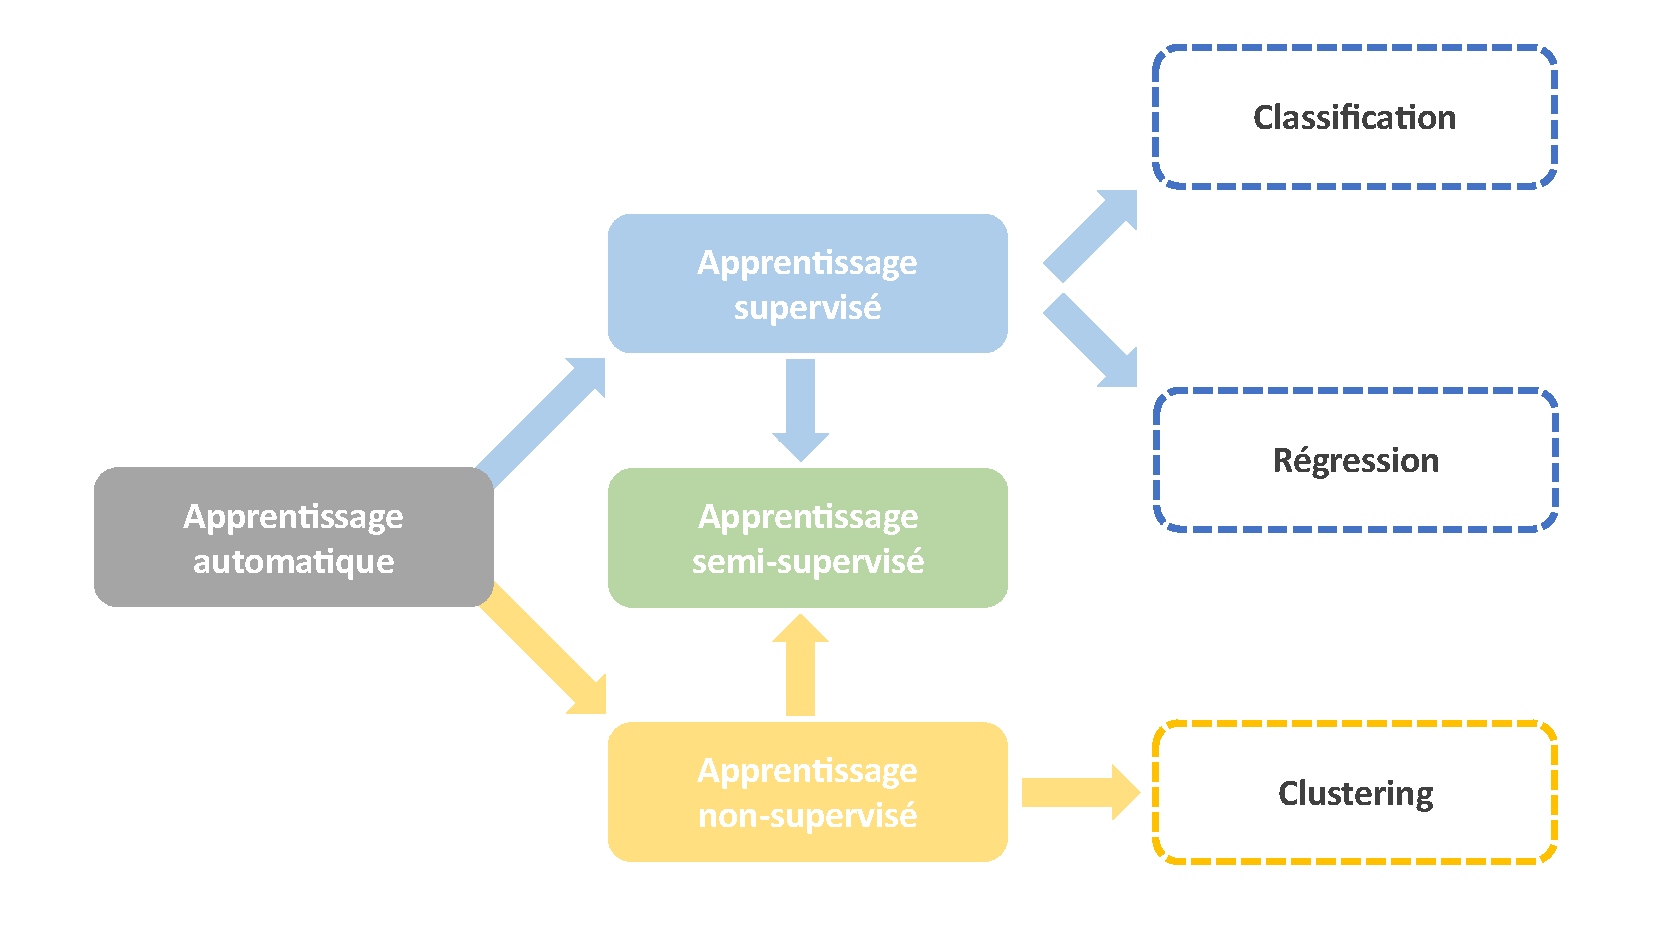
\includegraphics[width=\linewidth]{contents/chapter_3/resources/scheme_machine_learning.pdf}
    \caption{Schéma de décomposition des approches par apprentissage automatique.}
    \label{fig:scheme_machine_learning}
\end{figure}

\subsection{Apprentissage supervisé}
L’apprentissage supervisé ou « prédictif » consiste de manière simple à trouver une corrélation entre des données d’entrée $x$ et des sorties attendue $y$ et cela, dans le but de produire sur de nouvelles données d’entrée $x'$ de nouvelles sorties $y'$.\par

Cette approche implique l’utilisation d’une base d’apprentissage, définie comme « un ensemble de couples entrée-sortie » noté $\{(x_1,y_1 ),\ldots,(x_n,y_n )\}$ avec $n \in N$. Ainsi, l’humain tente de donner une signification aux données utilisées, pour lesquelles la machine devra être en mesure de trouver une corrélation.\par

L’algorithme tente de répondre au problème $y=f(x)$ où $f$ est notre fonction inconnue correspondant au phénomène observé, par une fonction d’approche $g$ appelée fonction de prédiction, tel que $y=g(x)$.\par 

Cet apprentissage, schématisé sur la \Cref{fig:scheme_supervised_classification}, se découpe en deux processus distincts :
\begin{itemize}
    \item D’une part, l’entraînement consistant à approcher la fonction $f$ par une fonction d’approche $g$,
    \item D’autre part, la prédiction consistant à prédire sur de nouvelles données à partir de $g$ tel que $g(x') = y'$.
\end{itemize}\par
  
\begin{figure}[H]
    \centering
    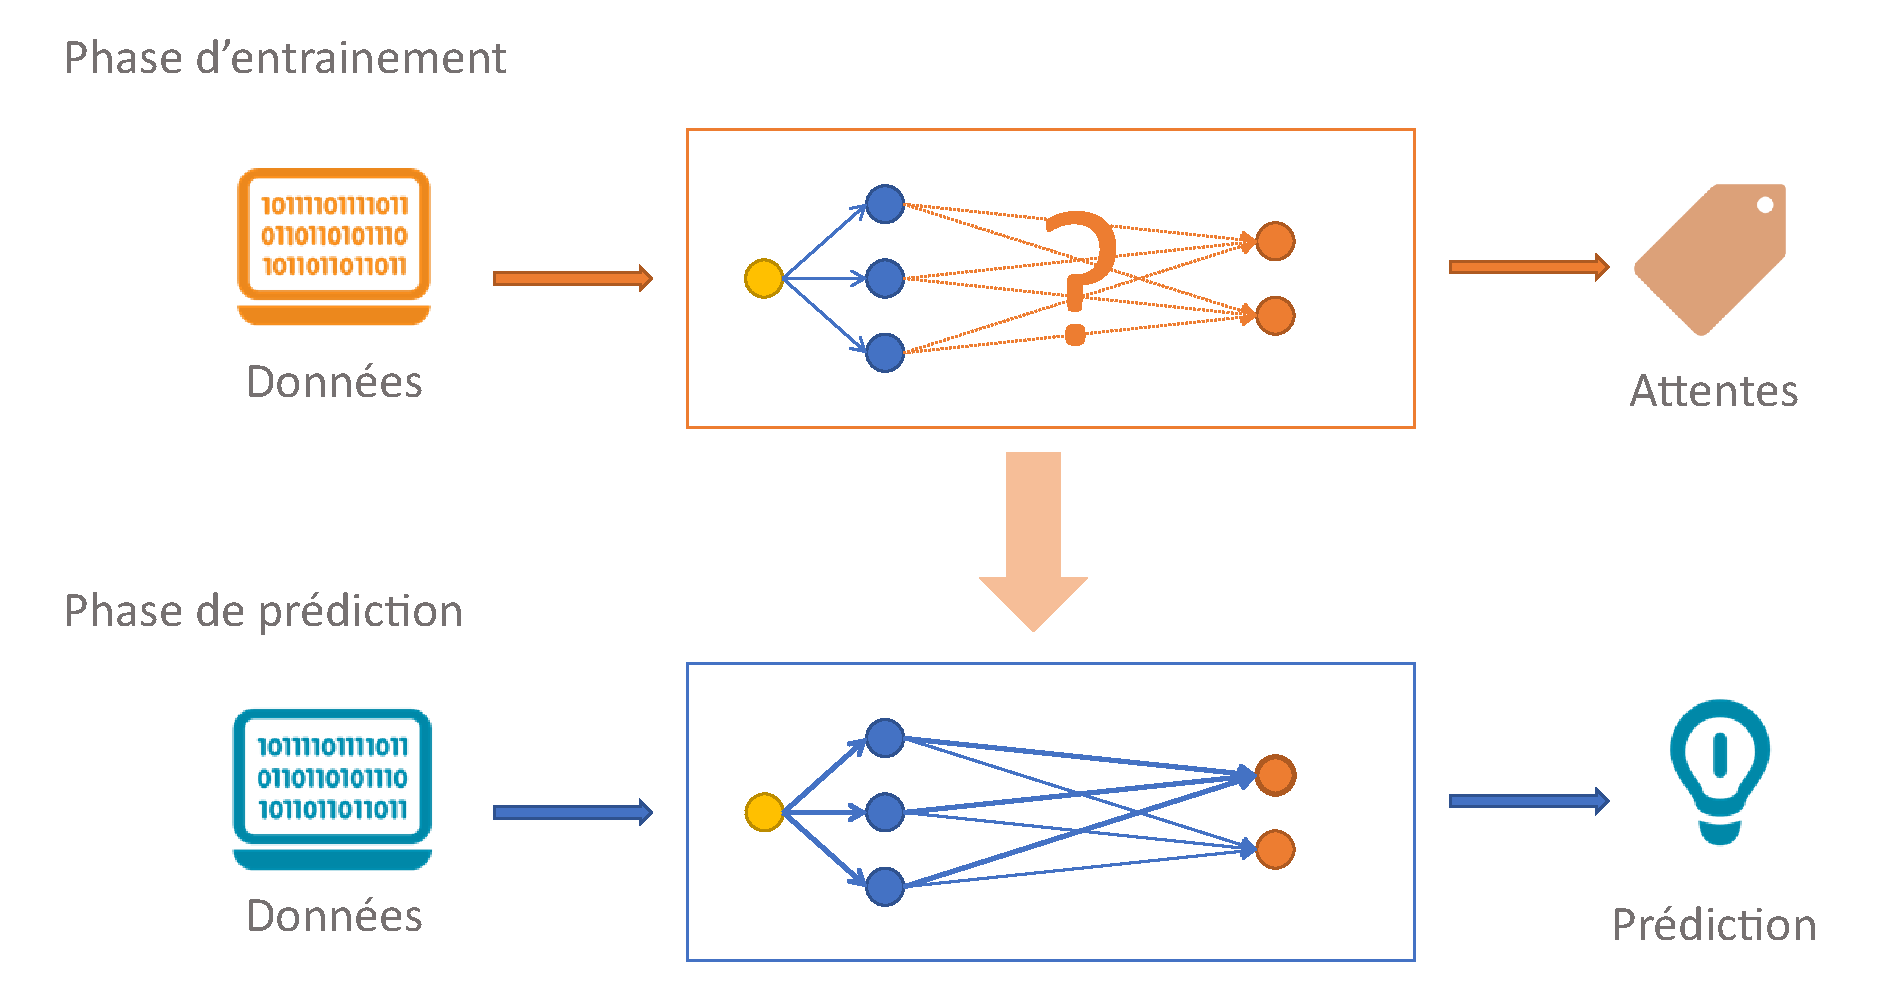
\includegraphics[width=0.8\linewidth]{contents/chapter_3/resources/scheme_supervised_classification.pdf}
    \caption{Schéma de l’approche dite supervisée. La phase d'entraînement va permettre de déterminer les relations entre données et attentes, sur des données connues dites d'apprentissages. La phase dé prédiction réutilisera les relation déterminées lors de la phase d'entraînement. }
    \label{fig:scheme_supervised_classification}
\end{figure}

Ces approches se regroupent au travers de deux types majeurs de résolution :
\begin{itemize}
    \item La prédiction de valeurs discrètes soit l’ensemble des entiers relatifs noté $\pmb{\mathbb{Z}}$, désignée sous le terme classification. Cette catégorie se subdivise en deux nouveaux types de classifications, qualifié de binaire ou de multi-classes lorsque la situation nécessite de prédire plus de deux valeurs.
    \item La prédiction de valeurs continues soit l’ensemble des nombres réels noté $\pmb{\mathbb{R}}$, désignée sous le terme de régression.
\end{itemize}\par

\subsection{Apprentissage non-supervisée}
L’apprentissage non supervisé ou « descriptif » est une seconde approche d’apprentissage dans laquelle l’ordinateur tente de « découvrir » en autonomie, des corrélations au sein de jeux de données. Ces approches émergent de problématiques diverses, telles que :
\begin{itemize}
    \item Réduire le coût, ou temps humain nécessaire, d’obtention de données étiquetées, c’est-à-dire pour lesquelles le couple de données d’entrée et de sortie attendue est connu.
    \item Découvrir les diverses relations pouvant exister au sein d’un amas de données. En effet, un label n’est qu’un échantillonnage de l’information primaire, et ne permet pas d’obtenir les relations pouvant régir des modèles complexes.
    \item Explorer de nouvelles relations de type « cause – effet », en réaction à la masse de données produites par les objets connectés. 
\end{itemize}\par

Plusieurs applications existent, telles que :
\begin{itemize}
	\item Le regroupement par classes, des algorithmes comme les k-moyennes tentent de minimiser la différence d’énergie entre les points d’un même groupe.
	\item La réduction de dimensions sur des données à grande complexité, par projection de ces dernières sur des espaces à dimension réduite. On souhaite par ce procédé garder l’information essentielle au processus décisionnel.
	\item La découverte de relations au sein de l’information, et des relations les plus robustes entre variables et dépendances.
\end{itemize}\par
 
\begin{figure}[H]
    \centering
    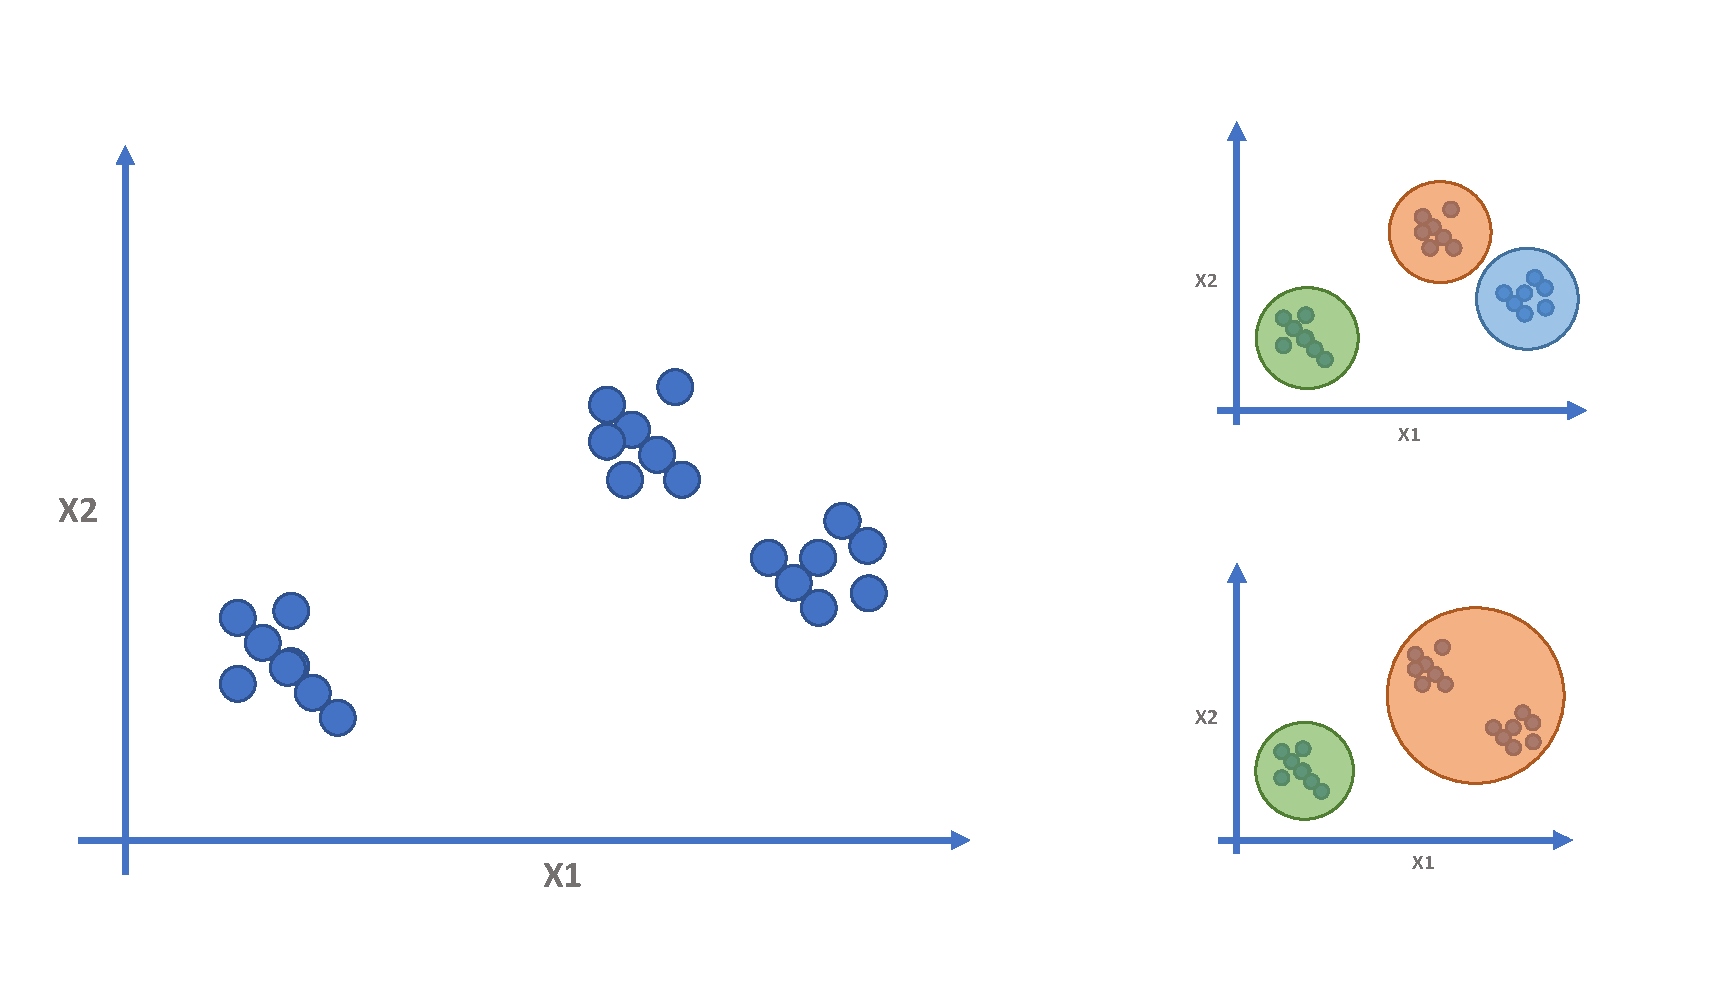
\includegraphics[width=0.8\linewidth]{contents/chapter_3/resources/scheme_unsupervised.pdf}
    \caption{Les données fournies ne sont pas associées à un label attendu. Nous demandons à la machine de découvrir des groupes de données (exemple avec 2 groupes et 3 groupes).}
    \label{fig:scheme_unsupervised}
\end{figure}

Ce principe a été également utilisé dans le but de réduire la dimension des données d'entraînement avant l'apprentissage supervisé. Cette technique porte le nom de sacs de mots ou "Bag-of-words" initialement prévue pour l'analyse de texte~\cite{Zhang2010} et utilisé dans des domaines tels que l'analyse d'image de la peau~\cite{Situ2008}.\par

\subsection{Apprentissage semi-supervisé}
Ces techniques tentent de combiner les deux principes précédents. Il est généralement difficile d’obtenir des données étiquetée en suffisance. D’une part, cela requiert le travail d’un opérateur sur ces données afin d’y associer les annotations adéquates. D’autre part, un grand nombre de données implique un possible biais humain dû à des erreurs sur ces annotations (manque d’attention, mauvaise interprétation de la donnée, …).\par

Par ce principe, les données étiquetées permettent de définir l'appartenance à des groupes des données, tandis que les données non étiquetées, permettent d’affiner les limites des groupes préalablement détectés (voir la \Cref{fig:scheme_semi_supervised}). Différentes techniques existent, basées sur des critères tels que la densité de l’information étiquetées et non étiquetées~\cite{chapelle2005}.\par
 
\begin{figure}[H]
    \centering
    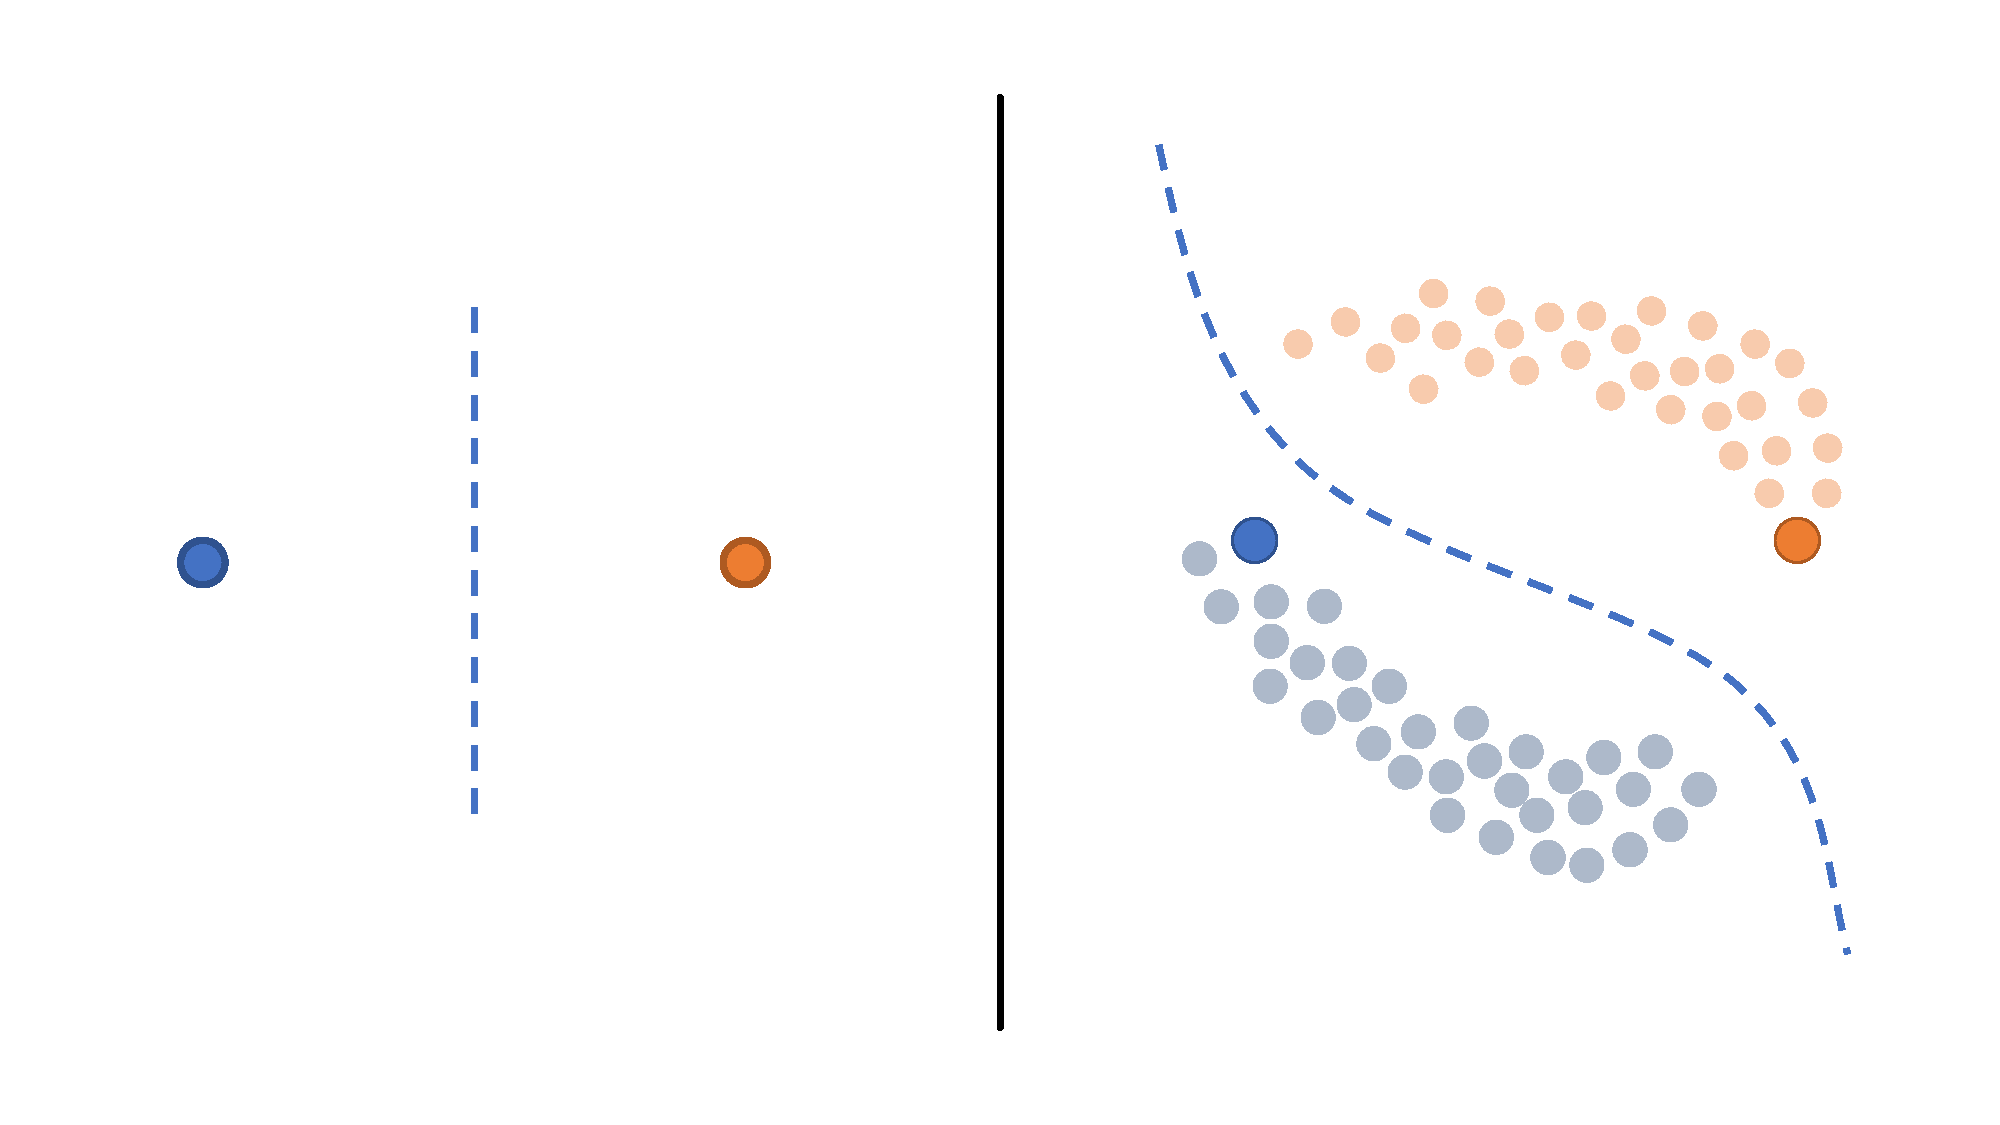
\includegraphics[width=\linewidth]{contents/chapter_3/resources/semi_supervised.pdf}
    \caption{A gauche, une classification obtenue à partir de deux données étiquetées, à droite ces mêmes données avec l’ajout de données non étiquetées. Ces nouvelles données sont alors attribuées à l’une ou l’autre des classes.}
    \label{fig:scheme_semi_supervised}
\end{figure}

\clearpage

\section{Apprentissage profond}
L’apprentissage profond correspond à un sous ensemble des méthodes d’apprentissage automatique qui tentent, par l’apports des neurosciences, de modéliser les schémas de fonctionnement du cerveau humain. Les derniers constats réalisés dans ce domaine, semblent démontrer que le cerveau possède divers niveaux de traitement de l’information . 
En effet, dans le cadre des méthodes « standard » d’apprentissage évoquées dans la partie précédente, la dimension de « couches » de traitement n’est pas intégrée. Les approches par apprentissage simple proposent une architecture en trois couches, dont l’une des couches est allouée à la corrélation entre nos données d’entrée et de sortie. Par opposition, les approches par apprentissage profond proposant des structures en n couches, avec $n \in \pmb{\mathbb{N}}$ et $n>1$.\par 

Ce choix d’architecture permet l’autodétermination de structures de caractéristiques complexes, définies par une combinaison non linéaire de caractéristiques plus simples. La \Cref{fig:scheme_dnn_understanding} met en évidence un cas plus simple de résolution par apprentissage pour appréhender cette notion. \par
 
\begin{figure}[H]
    \centering
    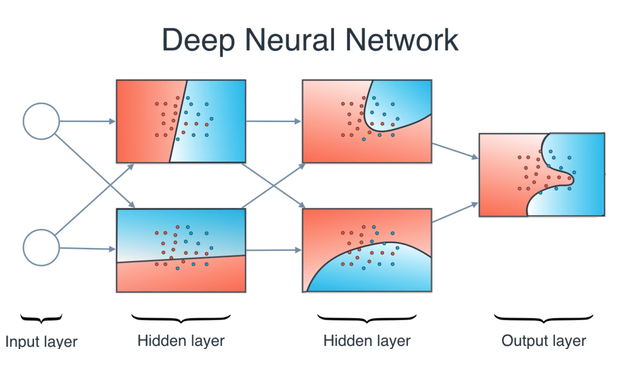
\includegraphics[width=\linewidth]{contents/chapter_3/resources/scheme_dnn_understanding.png}
    \caption{Exemple simplifié d'une structure d’apprentissage profond. Ce modèle se compose de deux couches intermédiaires cachées : la première couche extrait des caractéristiques linéaires simples, tandis que la seconde couche par combinaison à la première couche conduit à une extraction de caractéristiques plus complexes.}
    \label{fig:scheme_dnn_understanding}
\end{figure}

Ces solutions ont le désavantage de nécessiter des quantités de données non négligeables ainsi qu’une puissance de calcul, ou a contrario du temps, supérieur aux techniques d’apprentissage « simples ».
Plusieurs travaux ont été menés dans le domaine de la dermatologie pour permettre de déterminer la pertinence de ces méthodes. Nous retiendrons des thématiques autour de la reconnaissance du mélanome [24][25] largement abordé, ainsi que des travaux autour de la classification des lésions de natures diverses [26]. Ce dernier utilise un procédé de transfert de connaissance entre un réseau préalablement entraîné moins spécifique, et un nouveau réseau spécifique au problème de classification des lésions, dans le but de réduire le temps et les ressources nécessaires à l’entraînement du nouveau réseau.
Apprentissage par transfert
L’apprentissage par transfert est une discipline connexe à l’apprentissage profond défini comme « faisant référence à la situation où ce qui a été appris dans un contexte […] est exploité pour améliorer la généralisation dans une autre contexte » [27]. Cette discipline s’inscrit dans le champ de « l’adaptation de domaine », définie comme le transfert des connaissances d’un domaine $D_S$, défini par l’hypothèse $h: X_S \rightarrow Y_S$, vers un domaine cible $D_T$ afin de satisfaire $h: X_T \rightarrow Y_T$.
Ces solutions permettent de réduire les difficultés liées à la grande quantité de ressources de calcul, de temps, mais également de données mobilisées nécessaires à un entraînement depuis sa base. Le modèle d’apprentissage attendu est alors initialement plus performant, croît plus efficacement et plus performant qu’un apprentissage spécifique  (\Cref{fig:learning_curves}).

\begin{figure}[H]
    \centering
    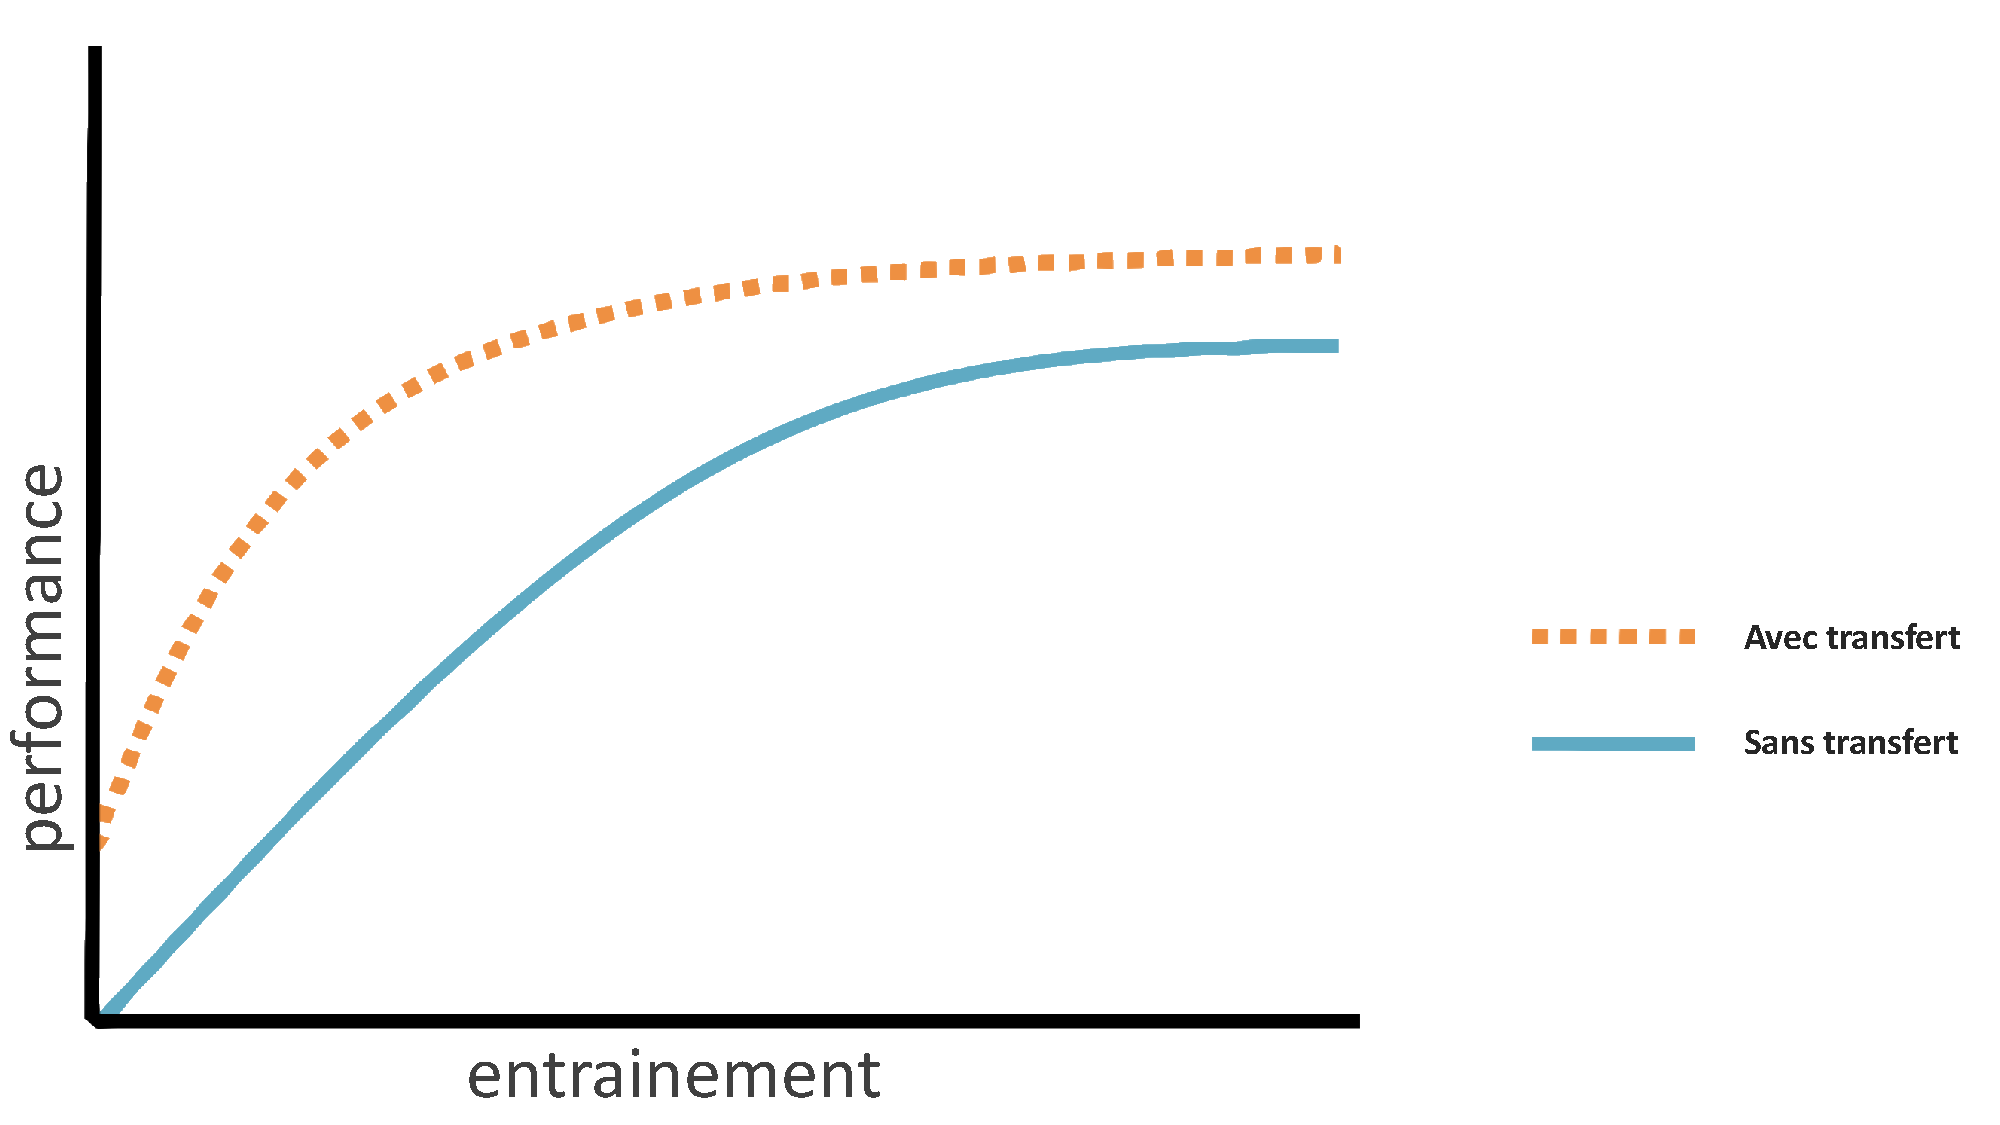
\includegraphics[width=\linewidth]{contents/chapter_3/resources/example_learning_curves.pdf}
    \caption{ Attentes liées à un apprentissage par transfert en opposition à un apprentissage classique.}
    \label{fig:learning_curves}
\end{figure}

Néanmoins, cette solution n’est envisageable que lorsque l’apprentissage, réalisé lors de la première tâche, généralise suffisamment le phénomène observé. Ainsi, il est d’usage courant de ne spécifier lors du transfert que la couche finale de classification du réseau, les premières couches n’étant employé comme extracteur général de caractéristiques. Toutefois, la littérature s’accorde sur une possible spécialisation des couches de classification et hautes moins génériques.
\subsection{Réseaux de neurones profonds}
\subsection{Réseaux neuronaux de convolutions}

\clearpage

\section{Réglages et évaluation de modèles prédictifs}
Cette partie se concentre sur des problématiques de biais lors de l'apprentissage et de l'évaluation de modèle. Nous tenterons de présenter rapidement le phénomène et les risques associées, puis nous proposerons des solutions permettant de s'affranchir d ces biais durant l'évaluation des modèles.\par

\subsection{Généralisation de modèles}
\label{subsec:generalized_models}
A l'aide de couples d'entrée/sortie préalablement possédée, nous allons tenter d’apprendre une relation capable de \textbf{généraliser} et d’estimer de nouvelles sorties sur de nouvelles données. Il est pour cela nécessaire de parvenir à isoler l'information responsable de ce cheminement, plus ou moins séparable, en cause souvent la qualité de :
\begin{inlinerate}
    \item l'hypothèse formulée, c'est à dire si la relation qui lie l'observation et sa conséquence est directe et vraie dans toutes circonstance,
    \item l'information possédée, c'est à dire si l'information est juste pour répondre à la problématique cible (qualité de l'observation, rapport signal sur bruit, etc.),
    \item \ldots.
\end{inlinerate}\par 

Ce problème, évoqué dans la littérature porte le nom de « dilemme biais / variance » , dans lequel le biais représente le manque de relation pertinente entre données d’entrées et de sorties et où la variance représente l’influence du modèle au petites fluctuations souvent issues de bruit. Ces termes sont intrinsèquement liés aux problématiques respectives de \textbf{sous-apprentissage} et \textbf{sur-apprentissage}. La \Cref{fig:example_underfit_overfit} reprend de manière visuelle ces problématiques, et les exprimes selon un jeu d’entraînement et de test. A noter que le sur-apprentissage peux être limité par l’utilisation de termes de régularisation, de schéma de validation de modèle adaptés ou l’utilisation d’ensembles de donnés suffisantes.\par
 
\begin{figure}[H]
    \centering
    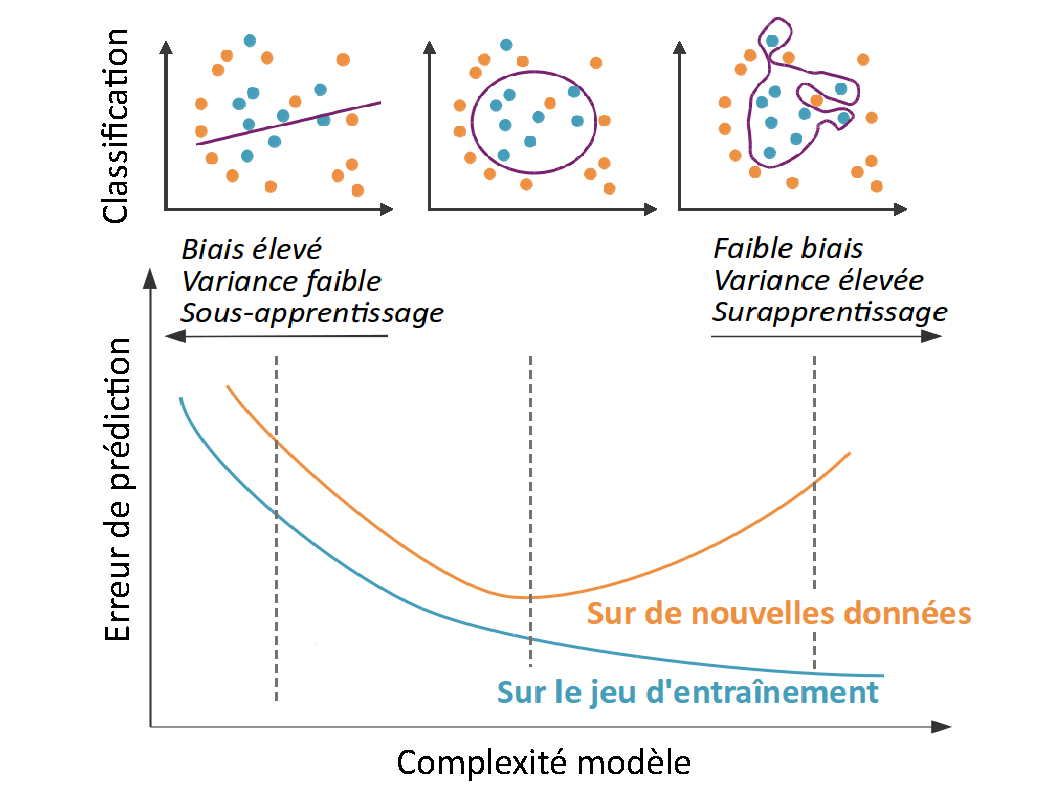
\includegraphics[width=0.8\linewidth]{contents/chapter_3/resources/example_underfit_overfit.pdf}
    \caption{Exemple de dilemme Biais/Variance. A gauche, un cas de sous-apprentissage, ce modèle est une sous approximation du phénomène observé. A droite, un cas de sur-apprentissage, le modèle ne généralise pas suffisamment le phénomène observé.}
    \label{fig:example_underfit_overfit}
\end{figure}

\subsection{Choix de métriques}
\label{subsec:metrics}
Le choix des métriques sont une part importante de nos problématiques lors de la mise en place de modèles d’apprentissage. En effet, il va permettre d'une part de déterminer la sélection d'un modèle parmi un ensemble de modèles et va permettre de retenir des performances attendues de ce dernier par exemple dans le monde réel.\par

L’un des principaux outils à disposition afin d'évaluer la performance est la matrice de confusion, schématisé sur la \Cref{fig:scheme_confusion_matrix}). Elle de faire correspondre les classes réelles et prédites : la diagonale de cette matrice fait figurer les prédictions correctement réalisées par notre modèle, tandis que les éléments restants nous renseignent sur les prédictions erronées. Dans une situation à deux classes ou \textit{binaire}, cette matrice fait ainsi ressortir quatre valeurs :
\begin{itemize}
	\item Les \textbf{vrais positifs}, les éléments de la classe positive détectés comme positif,
	\item Les \textbf{vrais négatifs}, les éléments de la classe négative détectés comme négatif,
	\item Les \textbf{faux positifs}, les éléments de la classe négative détectés comme positifs,
	\item Les \textbf{faux négatifs}, les éléments de la classe positive détectés comme négatifs.
\end{itemize}\par

\begin{figure}[H]
    \centering
    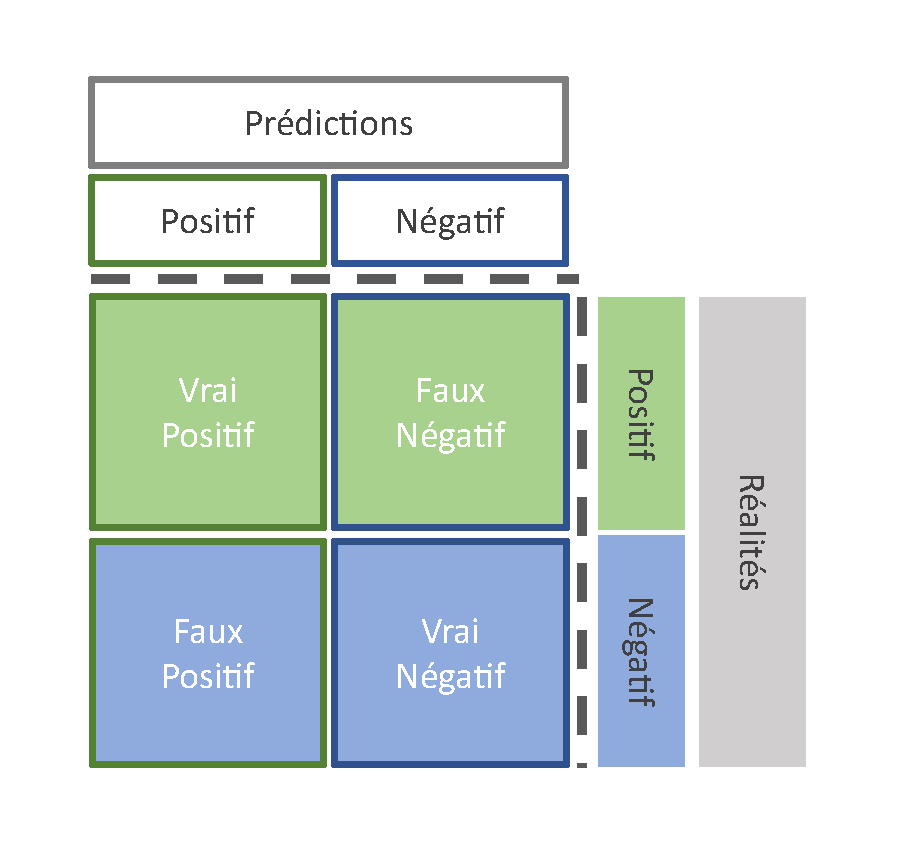
\includegraphics[width=0.6\linewidth]{contents/chapter_3/resources/scheme_confusion_matrix.pdf}
    \caption{Schéma représentatif d’une matrice de confusion, qui met en avant une situation binaire.}
    \label{fig:scheme_confusion_matrix}
\end{figure}

Bien que déjà réduite, l'information de cette matrice est encore très riche et difficile à utiliser comme critère de sélection. Pour cela, diverses métriques éprouvés seront à envisager selon la problématique à laquelle nous tenterons de répondre. Parmi les plus courant d'entre eux, les critères de précision, sensibilité ou encore spécificité sont pléthore dans la littérature mais ont tendance à ne capter qu'une partie du problème. Par exemple, la sensibilité est un critère très important en médecine ou détection de fraude, mais ne qualifie en rien la spécificité du modèle. De même, la moyenne fait également partie des critères extrait dans le domaine de l'intelligence artificielle, mais peux également manquer de sens en cas de non balancement de l'information~\cite{Guo2008} ou même ne pas mettre en avant un important gouffre entre spécificité et sensibilité. Ces métriques sont détaillés dans l'\Cref{eq:metrics_basics}.\par

\begin{equation} 
    \label{eq:metrics_basics}
    \begin{split}
    Sensibilit\acute{e} &= VP/(VP+FP) \\	
    Sp\acute{e}cificit\acute{e} &=  VN/(VN+FN) \\
    Pr\acute{e}cision &= VP/(VP+FP) \\
    Moyenne &= (VP+VN)/(VP+VN+FP+FN)
    \end{split}
\end{equation}

 Dans ce cas, il peut être préférable de privilégier des métriques plus robustes, dans le cadre de données non balancées. La plupart des méthodes s’accordent à l’utilisation de métriques tels que le F-Score, associant conjointement sensibilité et précision, par principe de la moyenne harmonique~\cite{Guo2008} (voir l'\Cref{eq:metrics_fscore}).\par
 
\begin{equation} 
    {F-Score}=(1+\beta^2)*(Pr\acute{e}cision*Sensibilit\acute{e})/((\beta^2*Pr\acute{e}cision)+Sensibilit\acute{e})
    \label{eq:metrics_fscore}
\end{equation}
 
Un autre métrique permettant de se prémunir de ces effets de non balancement de l'information et celui de l'\gls{auc} et découlant de la courbe \gls{roc}, dont le principe est résumé sur le schéma \Cref{fig:scheme_roc_curve}). La courbe \gls{roc} est tracée à partir des informations de spécificité / sensibilité et par variation d'une valeur seuil appliqué au modèle de prédiction, tandis que l'\gls{auc} correspond à l'intégration de l'aire de cette courbe. Ainsi, l'\gls{auc} est robuste au non balancement de données mais ses valeurs son optimiste sur des modèles de prédiction dont la variation du seuil est homogène vis à vis des résultats.\par

\begin{figure}[H]
    \centering
    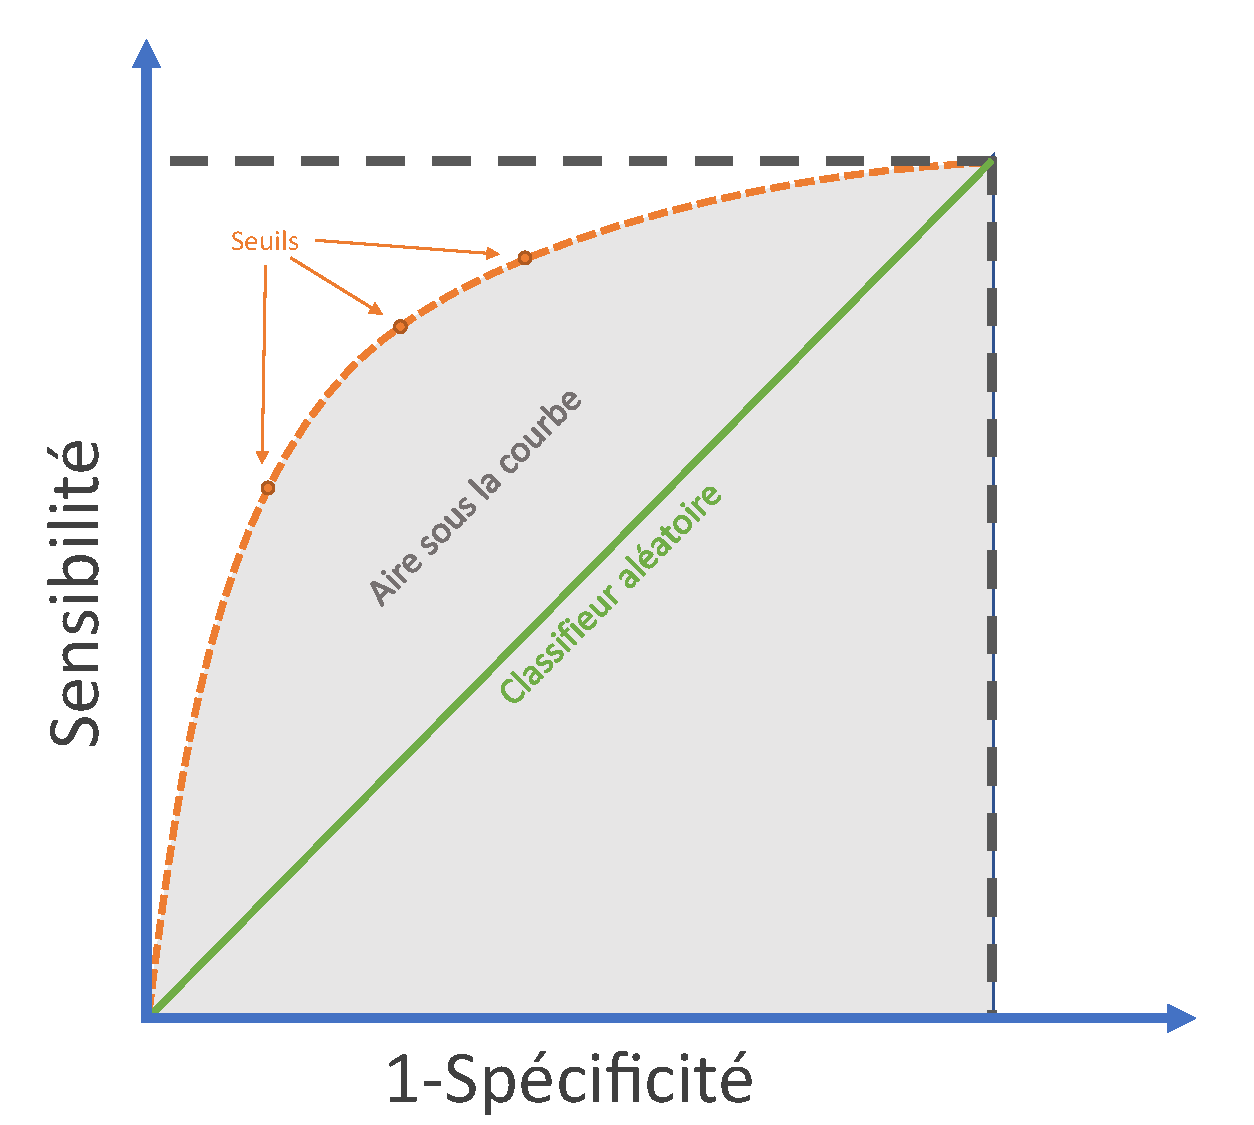
\includegraphics[width=0.6\linewidth]{contents/chapter_3/resources/scheme_roc_curve.pdf}
    \caption{Schéma de courbe \gls{roc} en orange et \gls{auc} en gris.}
    \label{fig:scheme_roc_curve}
\end{figure}

D'autres alternatives moins biaisé ont également été formulées~\cite{Sokolova2006}, néanmoins le F-Score et l'\gls{auc} sont couramment utilisé au sein des articles clinique et constituerons une des bases de notre travail.\par

\subsection{Réglages des hyperparamètres}
\label{subsec:hyperparameter}
Avant d’entrer plus en profondeur dans le sujet, il est nécessaire de revenir au terme « d’hyperparamètres ». Il caractérise les paramètres d'un processus d'apprentissage automatique dont le réglage doit être effectué avant le processus d’apprentissage, et dont le réglage dépendra des données à traiter mais ne pourra souvent être déterminé par la simple observation de celle-ci. Le réglage de ces hyperparamètres est ainsi difficile à appréhender et sera à refaire en fonction de chaque situation rencontrée.\par

L’une des premières techniques permettant ce réglage consiste à définir une « grille » de ces hyperparamètres, contenant pour chacun leurs possible variations~\cite{Liu2006}. Il s'agit de la méthode la plus équitable puisqu'elle consiste à évaluer chaque combinaisons, par comparaison des performances finales (voir la \Cref{fig:example_hyperparameter_selection} - Gauche). Néanmoins, elle possède deux limitations majeures, dont :
\begin{itemize}
    \item Son \textbf{temps de calcul}, qui va croître de manière exponentielle en fonction du nombre d'hyperparamètres à valider,
    \item Sa \textbf{précision}, qui va dépendre du pas choisi pour chacun des paramètres.
\end{itemize}\par

La seconde technique consiste à définir un « espace » de recherche dont la dilatation de chaque hyperparamètre sera choisie, ainsi qu'un nombre d'évaluation à réaliser pour déterminer la meilleure combinaison possible. Ce nombre d'évaluation est ensuite réalisé sous forme de tirage aléatoire, effectué à l'intérieur de cet espace de recherche défini~\cite{bergstra2012} (voir la \Cref{fig:example_hyperparameter_selection} - Droite). Cette méthode possède l'avantage d'être prévisible en terme de temps puisque le nombre de combinaisons évaluées est défini au préalable et quelque soit les proportions de l'espace. Néanmoins, cette méthode possède également des inconvénients comme la représentation des tirages au sein de l'espace défini.

\begin{figure}[H]
    \centering
    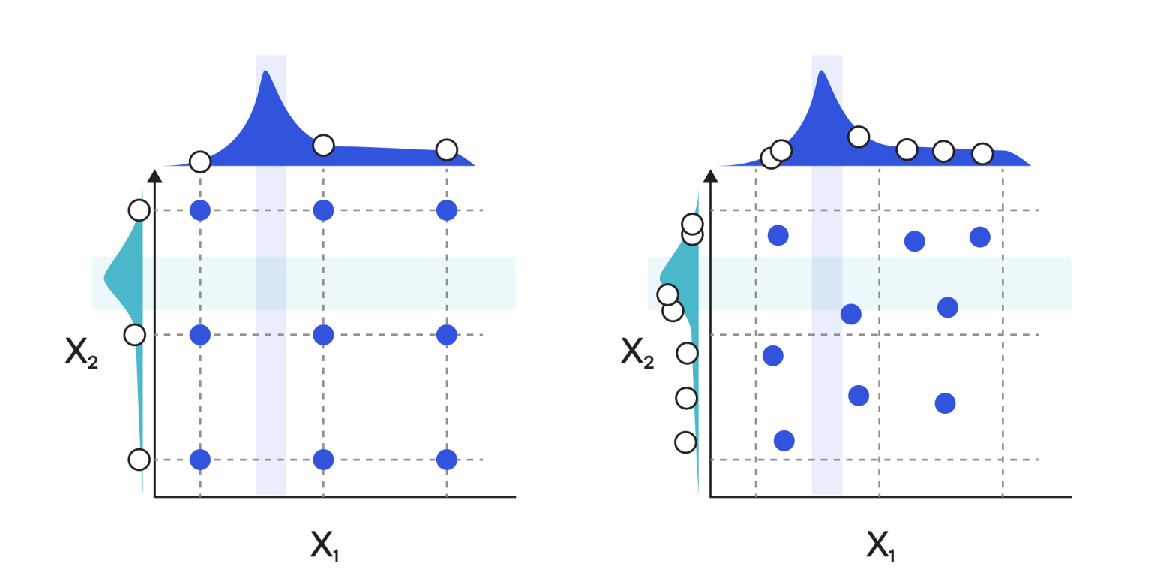
\includegraphics[width=\linewidth]{contents/chapter_3/resources/example_hyperparameter_selection.pdf}
    \caption{Exemple de recherche sur deux hyperparamètres $X_1$ et $X_2$. A gauche, une recherche sous forme de grille rigide, dans laquelle chaque combinaison sera évaluée. A droite, une recherche aléatoire de ces hyperparamètres.}
    \label{fig:example_hyperparameter_selection}
\end{figure}

\subsection{Méthodes d'évaluation}
Nous avons évoqué divers éléments permettant l'ajustement des modèles, voir la \Cref{subsec:hyperparameter}, et la mesure de performance, voir la \Cref{subsec:metrics}. Il est nécessaire d'orchestrer cet ensemble afin d'obtenir la meilleure attente possible d'un modèle de prédiction, tout en conservant une mesure permettant de renseigner sur la fiabilité de ce modèle et de ses prédictions futures dans des situations où la vérité terrain ne sera pas connue. En effet, l'évaluation d'un modèle de prédiction sur des données identiques à celles utilisées constitue un biais, par l'utilisation de connaissance à posteriori. De même, l'ajustement des hyperparamètres rentre dans cette catégorie de l'entraînement, et l'évaluation ne peut se faire sur des données ayant servi à les déterminer. Par ailleurs, une telle évaluation permet de détecter les problèmes de sous-apprentissage et sur-apprentissage évoqués en \Cref{subsec:generalized_models}.\par

La méthode \textbf{holdout} est la plus simple d'entre elle et consiste à diviser l’échantillon de données en deux sous-ensembles respectivement d'entraînement et de test. Il est important lors de cette étape de vérifier que les données présentes dans chacun de ces sous-ensembles soient représentatives de chaque classe présente dans la problématique. Les données spécifiées pour le test restent ainsi non utilisées jusqu'à leur confrontation au modèle définitif qui sera alors évalué par ces dernières. Le principal inconvénient de cette méthode est que seule une partie du jeu de donnée sert d'évaluation à la méthode développée. Néanmoins, cette méthode est rapide à exécuter puisqu'elle ne nécessite l'entraînement que d'un modèle. Cette méthode est schématisée sur la \label{fig:scheme_holdout_cv}, partie gauche.\par

La méthode de \textbf{validation croisée} permet d'étendre la méthode précédente à l'ensemble du jeu de données et d'obtenir un score moins biaisé. Pour cela, le jeu de données est subdivisé ainsi en \textbf{$k$ échantillons}, servant à tour de rôle de jeu de test, le reste de ces données étant réservé à l'entraînement. Nous obtenons ainsi $k$ modèles de prédictions et autant de score d'évaluation qui se résumerons à une unique valeur par application d'une fonction de moyenne. Le principal inconvénient de cette méthode est son de réalisation puisqu'elle nécessite l'entraînement d'autant de modèles que d'échantillons. Cette méthode est schématisée sur la \label{fig:scheme_holdout_cv}, partie droite.\par

\begin{figure}[H]
    \centering
    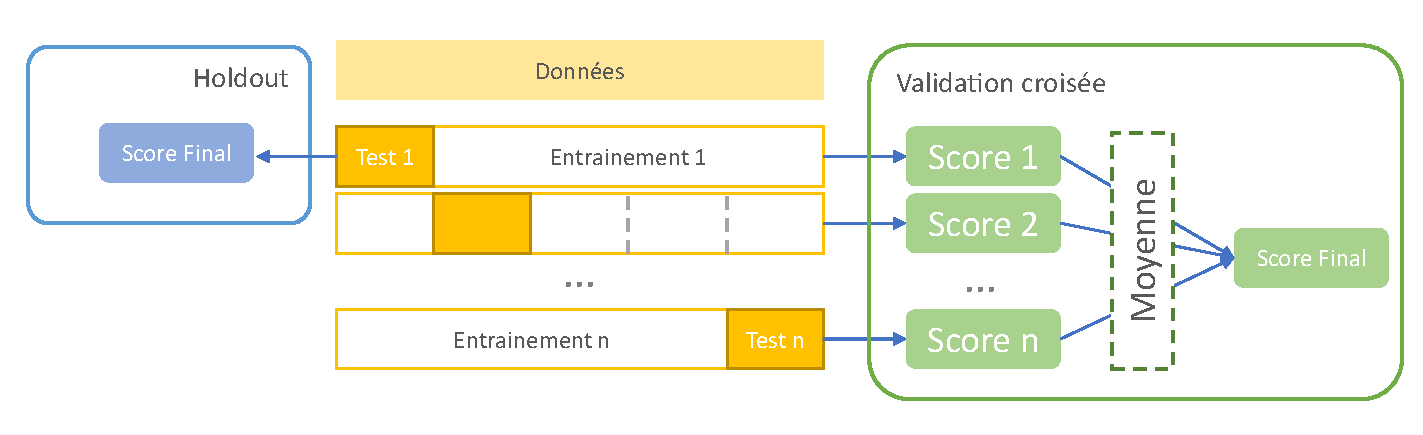
\includegraphics[width=\textwidth]{contents/chapter_3/resources/scheme_holdout_cv.pdf}
    \caption{Schéma des principes des deux approches majeures d'évaluation de modèles. A gauche, la méthode de « holdout » ; A droite, la méthode de validation croisée.}
    \label{fig:scheme_holdout_cv}
\end{figure}

Dans ce travail, nous nous intéresserons à la technique de validation croisée ainsi qu'à la valeur moyenne renvoyée par celle-ci. Afin de rendre l'information plus complète, nous renverrons également la valeur de déviation standard à partir des évaluations réalisé sur les divers échantillons, utilisée comme mesure de stabilité au sein de travaux statistiques~\cite{Kim2009}. La plupart des travaux employant la validation croisée emploie une valeur $k$ de 5, le choix de réduire cette valeur à 4 nous semble judicieux afin de réduire le temps de calcul tout en conservant une information cohérente.\par

Par ces deux méthodes nous répondons à la problématique de l'évaluation, mais n'apportons pas de solution quant au choix des hyperparamètres. En effet, utiliser un schéma de validation croisée pour régler et évaluer les modèles conduirait inévitablement à surestimer les performances du modèle~\cite{Tsamardinos2014}. Ce type de démarche reviendrait à ajuster au mieux une courbe à un nuage de points tout en affirmant que ces même données correspondent à des données inconnues. L'une des solutions a ce problème est l'utilisation d'un double schéma de validation, dont l'un des plus fonctionnels actuellement est celui de la validation croisée imbriquée~\cite{Cawley2010}. Le principe de cette méthode est schématisé sur la ~\Cref{fig:scheme_hyperparameter_process}, dans laquelle nous retrouvons :
\begin{itemize}
    \item une boucle \textbf{externe}, permettant d'évaluer un modèle à partir de données de \textbf{test},
    \item une boucle \textbf{interne}, permettant de valider un modèle et ses réglages à partir de données de \textbf{validation}.
\end{itemize}\par
  
\begin{figure}[H]
    \centering
    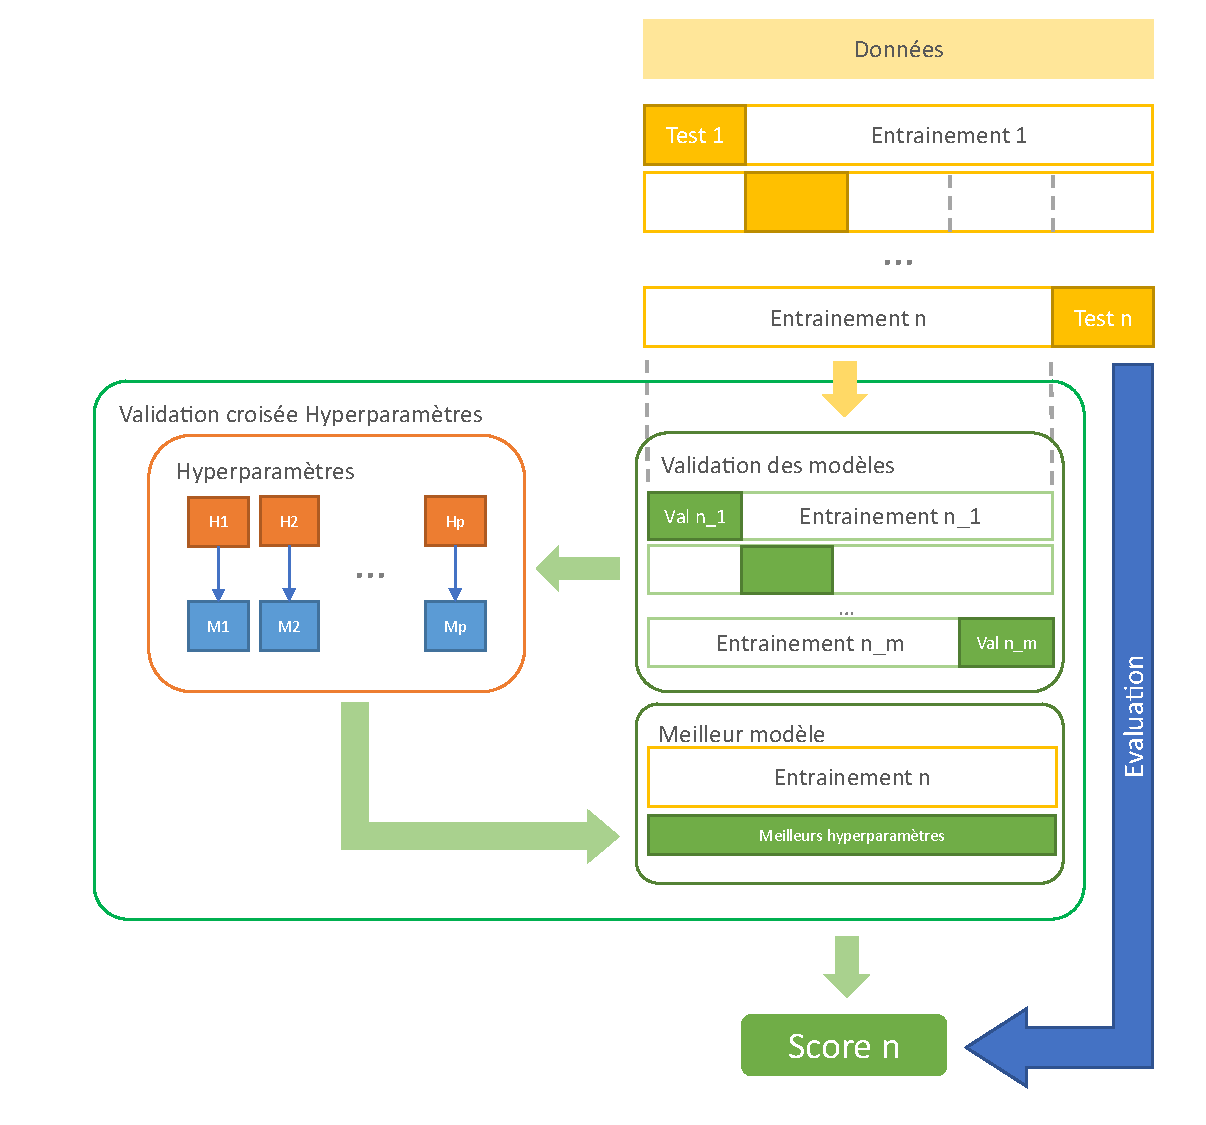
\includegraphics[width=\linewidth]{contents/chapter_3/resources/scheme_hyperparameter_process.pdf}
    \caption{Schéma de la validation croisée imbriquée assurant le choix de la meilleur combinaison d'hyperparamètres et assurant une évaluation robuste des performances du modèle.}
    \label{fig:scheme_hyperparameter_process}
\end{figure}

\clearpage

\section{Fusion d’informations}
Dernier aspect de notre sujet, la fusion d’informations se définie comme l’action de "combiner des informations issues de plusieurs sources afin d’améliorer la prise de décision" ~\cite{Bloch2003}. Cette fusion se retrouve dans de nombreux domaines d'applications dont celui de la santé ou encore de la biométrie, et peux être considéré comme un moyen d'augmenter la fiabilité de systèmes. L'intérêt croissant pour ce domaine correspond, entre autre, à une réponse de l'augmentation et de la diversification du nombre de capteurs présent. L'ouvrage de Bloch~\cite{Bloch2003} justifie la fusion d'information, par différentes notions auxquelles sont soumises chaque capteurs, dont:
\begin{itemize}
    \item \textbf{l'incertitude} : c'est à dire son "degré de conformité avec la réalité".
    \item \textbf{l'imprécision} : définie comme une "mesure du défaut quantitatif de connaissance, sur une mesure".
    \item \textbf{l'incomplétude} : correspond à "l'absence d'information d'une source sur des aspects du problème".
\end{itemize}\par

Cette fusion est indispensable pour permettre la réalisation de certaines tâches, l'effet de McGurk est un exemple concret de la \textit{complémentarité} de la vision et de l'audition dans le rôle de la perception de la parole, mais également de la difficulté à gérer les \textit{conflits} d'informations sur ces deux sources séparées~\cite{Mcgurk1976}. L'ouvrage de Bloch~\cite{Bloch2003} définie 3 termes propre à cette fusion:
\begin{itemize}
    \item \textbf{Le conflit} : l'une des notions pouvant conduire à de mauvaise interprétation de la part de systèmes lorsque plusieurs information contradictoires sont reçues.
    \item \textbf{La redondance} : l'apport multiple d'une même information, pouvant dans l'idéal permettre de réduire les incertitudes et les imprécisions.
    \item \textbf{La complémentarité} : généralement des sources, liée à un apport de caractéristiques différentes permettant l'accès à une information globale et de lever des ambiguïtés.
\end{itemize}\par

Il est nécessaire également de caractériser le résultat de la fusion d'information
Il est relativement difficile d'obtenir une vision commune sur les divers niveaux et termes associés. Ainsi, ce travail se réfère à l'une d'entre elle~\cite{Dasarathy1997} proche de notre problématique. Trois niveaux de fusion y sont décrit:
\begin{itemize}
\item le niveau bas ou celui des données,
\item le niveau moyen ou celui liés à des caractéristiques / des données de plus haut niveau,
\item le niveau haut ou celui des décisions.
\end{itemize} Niveaux au sein desquels le processus de fusion d'information peux aboutir à :
\begin{inlinerate}
\item une sélection,
\item une transformation,
\item une extraction,
\item ou encore une classification de l'information.
\end{inlinerate} La \Cref{fig:scheme_overview_fusion} propose une schématisation macroscopique de ce concept.\par
 
\begin{figure}[H]
    \centering
    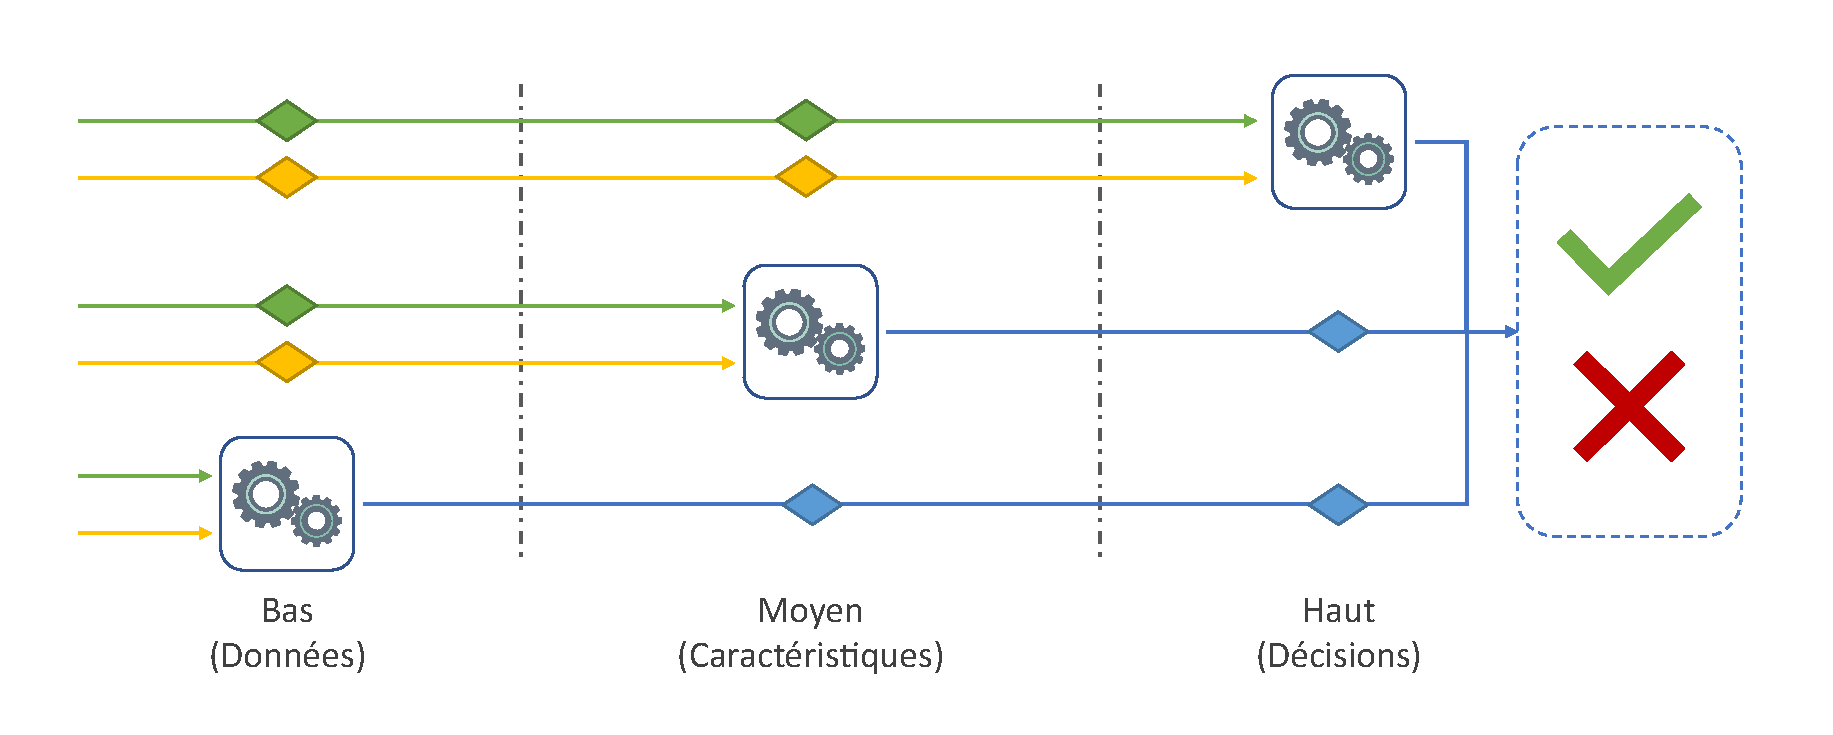
\includegraphics[width=\linewidth]{contents/chapter_3/resources/scheme_overview_fusion.pdf}
    \caption{Schéma des différents niveaux théoriques de fusion sur un schéma multimodal à deux capteurs. Le niveau bas représente le niveau le plus proche des données et du capteurs, le niveau moyen représente le niveau aux plus proche de l'extraction de caractéristiques avancées, enfin le niveau haut représente le niveau de prise de décision.}
    \label{fig:scheme_overview_fusion}
\end{figure}\par

La fusion à \textbf{bas niveau} s'exerce au niveau du capteur, quand celui-ci bénéficie de plusieurs relevés d'informations physique, ou après l'acquisition de données provenant de plusieurs capteurs. Cela va nécessiter une cohérence entre ces modalités: un référentiel, un repère commun permettant la mise en parallèle de ces dernières. La fusion à ce niveau consistera essentiellement à fournir une cohérence de ces modalités d'information, voir à réduire cette dernière afin de n'obtenir que celle jugée pertinente dans le cadre de son utilisation.\par

La fusion à \textbf{moyen niveau} s'exerce au niveau de caractéristiques, c'est à dire après un premier traitement de chacune des modalités pour n'extraire que les éléments nécessaire à la réalisation du processus. Il s'agit d'une mise en commun des vecteurs d'information dans leur totalité ou réduite nécessitant dans ce second cas une sélection de l'information pertinente.\par

Enfin, la fusion à \textbf{haut niveau} s'exerce après les mécanismes de prise de décision. C'est à dire que les branches correspondant à chaque modalité exercent indépendemment leur prise de décision. Il est donc nécessaire de définir une stratégie permettant de privilégier une décision ou d'extraire une décision à partir de l'information. Deux catégories sont ainsi identifiables: 
\begin{inlinerate}
\item la \textbf{sélection dynamique de modèle} de prédiction dans lequel l'objectif est de définir le modèle pertinent,
\item et la \textbf{fusion de modèles} de prédiction dans lequel le but est d'obtenir une décision globale tenant compte des différentes décisions.
\end{inlinerate}\par

Plus particulièrement, dans le cadre de problématique binaire, la fusion de modèle comporte deux niveaux conceptuels de décisions basées sur le type d'information mise à disposition par ces modèles. D'une part, au plus haut niveau : la fusion appliquée au \textbf{niveau décisionnel}. Seule les décisions issues de chaque modèle sont alors considérées selon diverses stratégies: le vote à la majorité ou encore la pondération des votes en sont deux représentants. D'autre part, au plus bas niveau : la fusion appliquée aux scores~\cite{Kittler1998}. Dans le cadre de problématique à plusieurs classes, nous pouvons évoquer une troisième prise de décision au niveau du rang, c'est à dire en considérant la position de chaque classe prédite issue des divers modèles.\par


% Ce terme caractérise, dans le cadre de ce travail, les approches d’intelligence artificielle n’appartenant pas au cadre de l’apprentissage automatique. Il s’agit d’approches dont la succession de règles, ou des traitements pas à pas, est définie par un humain. Cette démarche fait suite aux travaux de Turing, décrivant que tout problème peut se résoudre par une suite d’étapes successives \cite{Turing1937}. L’ordinateur ne cherchera pas à comprendre la relation entre les données d’entrée et attendues en sortie, mais appliquera les divers traitements qui lui ont été demandés.\par



% Ces solutions proposent ainsi des règles statiques et nécessitent une révision de toute ou partie du processus lorsque les données d’entrées sont vouées à varier. De plus, ces approches peuvent être dépassées en cas d’une grande diversité des données d’entrée.\par
 
% \begin{figure}[H]
%     \centering
%     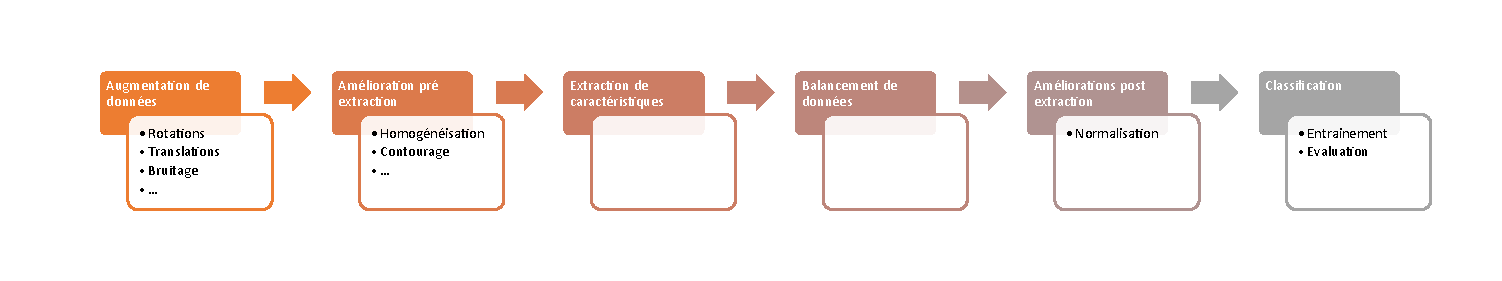
\includegraphics[width=\linewidth]{contents/chapter_3/resources/classic_pipeline.pdf}
%     \caption{Schématisation d’une approche par algorithme.}
%     \label{fig:standard_process}
% \end{figure}\par

% La littérature traitant de « la détection de lésions de la peau » est assez peu développée pour ces approches « algorithmiques » \cite{Moss1989}. Les approches par apprentissage, dont nous allons aborder les grandes lignes dans la section suivante, ont grandement contribué au développement de cette thématique dans la littérature scientifique.\par   

% \subsubsection{Détection d'anomalies}
% Cette technique est particulièrement propice aux données représentant majoritairement les cas définis comme « normaux », et pour lesquels nous souhaitons détecter les cas « aberrants ». En 1980, Douglas Hawkins apporte la définition d’une valeur aberrante comme « Une observation qui s’écarte tellement des autres observations, qu’elle éveille le soupçon d’avoir été généré par un mécanisme différent ». Diverses méthodes existent, dont l’une des plus utilisées se base sur une distribution gaussienne, excluant les valeurs qualifiées d’extrême déterminée par un seuil $\varepsilon$ (Figure 35). Gaussian mixture model.
  
% \begin{figure}[H]
%     \centering
%     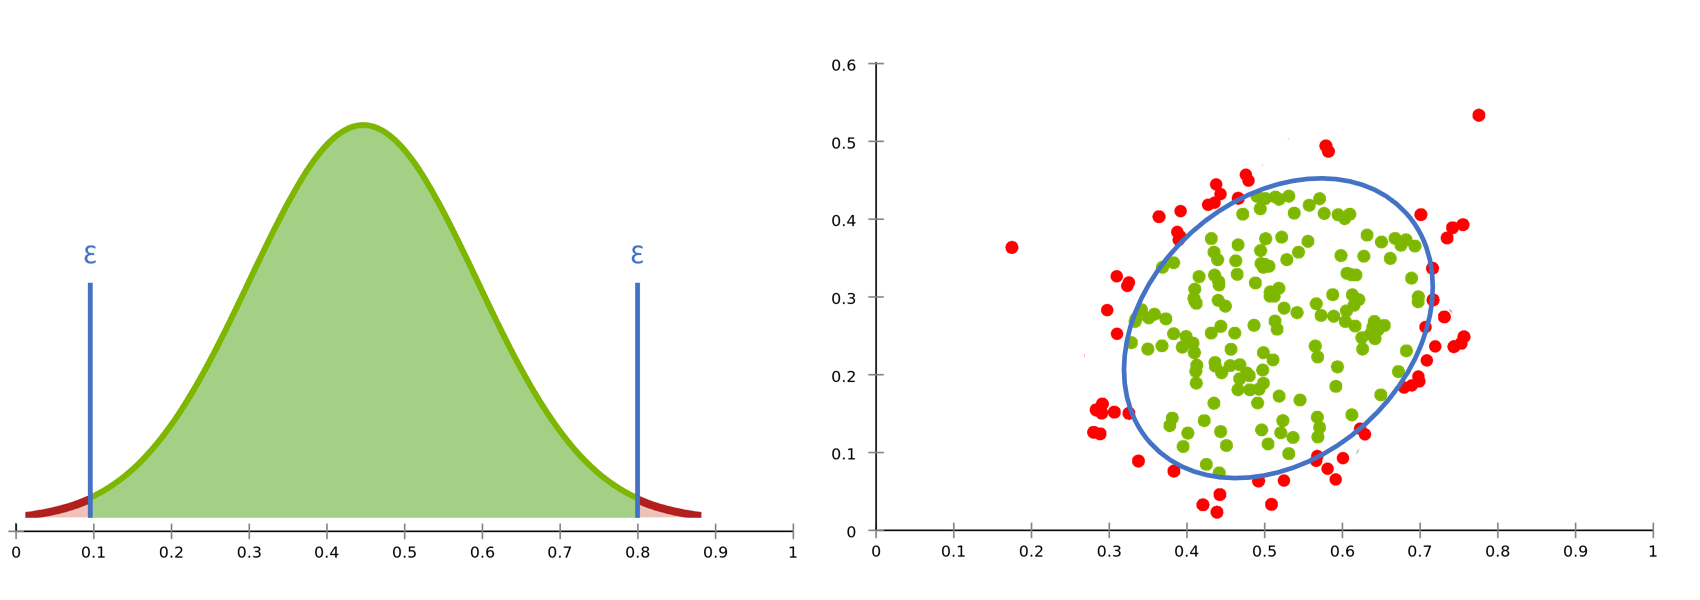
\includegraphics[width=\linewidth]{contents/chapter_3/resources/anomaly_detection.png}
%     \caption{Exemple sur des données arbitraires. Un seuil $\varepsilon$ (en bleu) est déterminé à partir des moyennes et écart type des données.}
%     \label{fig:anomaly_detection}
% \end{figure}

% \subsection{Équilibrage de données}
% Nous regroupons au travers de ce terme l’ensemble des problématiques relatives à notre jeu de données et à la représentation de ses classes. Dans le cas de pathologie de la peau, cela peut se caractériser par un jeu de données composé de 100 éléments dont 20\% d’entre elles se réfèrent à des patients atteints de mélanomes et le reste à des patients sains. Nous constatons dans ce cas un déséquilibre entre les classes de ce jeu de données, qu’il nous faudra prendre en compte. Un tel jeu de données peut être qualifié de « non balancés », la répartition de ses classes n’étant pas égale en proportions.
% En effet, certains algorithmes de prédictions peuvent être biaisés, comme par exemple « l’algorithme des plus proches voisins » qui se composera de zones de forte densité privilégiant les données présentes en masse (exemple Figure 37). Un autre biais est également présent lors de l’extraction de métriques pour juger de la pertinence d’un modèle. En effet, dans le cas d’un classifieur qui prédirait constamment « sain », nous obtiendrons un score de 80\% de précision sur notre jeu de données précédent.
  
% \begin{figure}[H]
%     \centering
%     \includegraphics[width=\linewidth]{contents/chapter_3/resources/unbalanced.pdf}
%     \caption{Illustration du problème de données non balancées sur l’algorithme KNN. La densité des données bleu étant supérieure, des prédictions à la frontière de nos deux classes favorisent la classe bleue.}
%     \label{fig:unbalanced}
% \end{figure}

% Plusieurs méthodes existent dans la littérature, pour permettre de rétablir l’équilibre entre les différentes classes. Nous pouvons citer les deux principaux :
% 	Le sur-échantillonnage, c’est-à-dire que nous gonflons les classes sous représentatives de manière à égaliser la population de la classe majoritaire (en créant de nouveaux éléments artificiels par exemple).
% 	Le sous-échantillonnage, c’est-à-dire que nous réduisons la population de l’ensemble des classes à celle de la classe minoritaire.
 
% \begin{figure}[H]
%     \centering
%     \includegraphics[width=\linewidth]{contents/chapter_3/resources/example_balancement_strategies.pdf}
%     \caption{Représentation de deux principales catégories de stratégie de balancement des données. Le suréchantillonnage tente d’augmenter la taille du jeu de données faible tandis que le sous échantillonnage tend à réduire la classe majoritaire. }
%     \label{fig:example_balancement_strategies}
% \end{figure}